% Options for packages loaded elsewhere
\PassOptionsToPackage{unicode}{hyperref}
\PassOptionsToPackage{hyphens}{url}
\PassOptionsToPackage{dvipsnames,svgnames,x11names}{xcolor}
%
\documentclass[
  11pt,
  letterpaper,
]{scrreprt}

\usepackage{amsmath,amssymb}
\usepackage{iftex}
\ifPDFTeX
  \usepackage[T1]{fontenc}
  \usepackage[utf8]{inputenc}
  \usepackage{textcomp} % provide euro and other symbols
\else % if luatex or xetex
  \usepackage{unicode-math}
  \defaultfontfeatures{Scale=MatchLowercase}
  \defaultfontfeatures[\rmfamily]{Ligatures=TeX,Scale=1}
\fi
\usepackage{lmodern}
\ifPDFTeX\else  
    % xetex/luatex font selection
  \setmainfont[]{Calibri}
\fi
% Use upquote if available, for straight quotes in verbatim environments
\IfFileExists{upquote.sty}{\usepackage{upquote}}{}
\IfFileExists{microtype.sty}{% use microtype if available
  \usepackage[]{microtype}
  \UseMicrotypeSet[protrusion]{basicmath} % disable protrusion for tt fonts
}{}
\makeatletter
\@ifundefined{KOMAClassName}{% if non-KOMA class
  \IfFileExists{parskip.sty}{%
    \usepackage{parskip}
  }{% else
    \setlength{\parindent}{0pt}
    \setlength{\parskip}{6pt plus 2pt minus 1pt}}
}{% if KOMA class
  \KOMAoptions{parskip=half}}
\makeatother
\usepackage{xcolor}
\setlength{\emergencystretch}{3em} % prevent overfull lines
\setcounter{secnumdepth}{5}
% Make \paragraph and \subparagraph free-standing
\ifx\paragraph\undefined\else
  \let\oldparagraph\paragraph
  \renewcommand{\paragraph}[1]{\oldparagraph{#1}\mbox{}}
\fi
\ifx\subparagraph\undefined\else
  \let\oldsubparagraph\subparagraph
  \renewcommand{\subparagraph}[1]{\oldsubparagraph{#1}\mbox{}}
\fi


\providecommand{\tightlist}{%
  \setlength{\itemsep}{0pt}\setlength{\parskip}{0pt}}\usepackage{longtable,booktabs,array}
\usepackage{calc} % for calculating minipage widths
% Correct order of tables after \paragraph or \subparagraph
\usepackage{etoolbox}
\makeatletter
\patchcmd\longtable{\par}{\if@noskipsec\mbox{}\fi\par}{}{}
\makeatother
% Allow footnotes in longtable head/foot
\IfFileExists{footnotehyper.sty}{\usepackage{footnotehyper}}{\usepackage{footnote}}
\makesavenoteenv{longtable}
\usepackage{graphicx}
\makeatletter
\def\maxwidth{\ifdim\Gin@nat@width>\linewidth\linewidth\else\Gin@nat@width\fi}
\def\maxheight{\ifdim\Gin@nat@height>\textheight\textheight\else\Gin@nat@height\fi}
\makeatother
% Scale images if necessary, so that they will not overflow the page
% margins by default, and it is still possible to overwrite the defaults
% using explicit options in \includegraphics[width, height, ...]{}
\setkeys{Gin}{width=\maxwidth,height=\maxheight,keepaspectratio}
% Set default figure placement to htbp
\makeatletter
\def\fps@figure{htbp}
\makeatother

\usepackage{fontspec}
\usepackage{xcolor}
\usepackage{graphicx}
\usepackage{eso-pic}
\usepackage{changepage}
\usepackage{tikz}
\usepackage{sectsty}
\usepackage{typearea}
\usepackage{pdflscape}
\usepackage{hyperref}
\usepackage{ulem} % Pour le sous-lignage

\usepackage{titlesec}
\definecolor{color_orange}{RGB}{227,108,10} % Définit la couleur orange foncé du chapitre
\definecolor{color_grey}{RGB}{128,128,128} % Définit la couleur grise du titre partie
\definecolor{color_purple}{RGB}{102,0,102} % Définit la couleur mauve pour le titre sous partie.
\definecolor{color_black}{RGB}{0,0,0} % Définit la couleur mauve pour le titre sous partie.

\definecolor{head_color}{RGB}{250,192,144} % Définit la couleur orange clair pour l'en tête.

\usepackage[a4paper, margin=1in]{geometry} % Configure les marges de la page

% modification de l'en-tête
\usepackage[automark]{scrlayer-scrpage}
\clearpairofpagestyles % Efface les configurations d'en-tête et de pied de page par défaut
\ihead{Analyse spatiale de l’impact environnemental des incendies de 2021 sur la Nouvelle-Calédonie} %titre du document
\addtokomafont{pagehead}{\normalfont\fontsize{8pt}{10pt}\selectfont} %taille de l'en-tête
\addtokomafont{pagehead}{\color{head_color}} % couleur de l'en-tête 

% modification du pied de page

\ifoot{Observatoire de l’environnement en Nouvelle-Calédonie. OEIL \\
12 rue Tourville 98800 Nouméa - Tél. / Fax : 23 69 69 - \href{http://www.oeil.nc}{www.oeil.nc}} % Pied de page à gauche
\addtokomafont{pagefoot}{\normalfont\fontsize{8pt}{10pt}\selectfont} % taille du pied de page
\addtokomafont{pagefoot}{\color{color_grey}} % couleur du pied de page

% modification de la position des numéro de page
\cfoot*{} 
\ofoot*{\pagemark} 
\setkomafont{pagenumber}{\normalfont} % numéro des pages 

\usepackage{float}
\floatplacement{table}{H}  %positionne les tableaux comme défini dans le script

\renewcommand{\thesection}{\Roman{section}}
\renewcommand{\thesubsection}{\thesection.\arabic{subsection}}
\renewcommand{\thesubsubsection}{\thesubsection.\arabic{subsubsection}}
\renewcommand{\theparagraph}{\thesubsubsection.\alph{paragraph}}
\renewcommand{\thesubparagraph}{\roman{subparagraph}.\hspace{1.5em}}

%modification des titres pour appliquer la version OEIL
\titleformat*{\section}{\normalfont\fontsize{14pt}{19pt}\selectfont\color{color_orange}} % chapitre
\titleformat*{\subsection}{\normalfont\fontsize{12pt}{19pt}\selectfont\color{color_grey}} % Titre partie
\titleformat*{\subsubsection}{\normalfont\fontsize{11pt}{19pt}\selectfont\bfseries\itshape\color{color_purple}} %titre sous partie
\titleformat*{\paragraph}{\normalfont\fontsize{11pt}{19pt}\selectfont\bfseries\itshape\color{color_black}} %titre sous partie
\titleformat*{\subparagraph}{\normalfont\fontsize{11pt}{19pt}\selectfont\itshape\color{color_black}} %titre sous partie
\titlespacing*{\subparagraph}{2em}{1.25ex plus 10ex minus .1ex}{\baselineskip}
\makeatletter
\@ifpackageloaded{bookmark}{}{\usepackage{bookmark}}
\makeatother
\makeatletter
\@ifpackageloaded{caption}{}{\usepackage{caption}}
\AtBeginDocument{%
\ifdefined\contentsname
  \renewcommand*\contentsname{Table of contents}
\else
  \newcommand\contentsname{Table of contents}
\fi
\ifdefined\listfigurename
  \renewcommand*\listfigurename{List of Figures}
\else
  \newcommand\listfigurename{List of Figures}
\fi
\ifdefined\listtablename
  \renewcommand*\listtablename{List of Tables}
\else
  \newcommand\listtablename{List of Tables}
\fi
\ifdefined\figurename
  \renewcommand*\figurename{Figure}
\else
  \newcommand\figurename{Figure}
\fi
\ifdefined\tablename
  \renewcommand*\tablename{Table}
\else
  \newcommand\tablename{Table}
\fi
}
\@ifpackageloaded{float}{}{\usepackage{float}}
\floatstyle{ruled}
\@ifundefined{c@chapter}{\newfloat{codelisting}{h}{lop}}{\newfloat{codelisting}{h}{lop}[chapter]}
\floatname{codelisting}{Listing}
\newcommand*\listoflistings{\listof{codelisting}{List of Listings}}
\makeatother
\makeatletter
\makeatother
\makeatletter
\@ifpackageloaded{caption}{}{\usepackage{caption}}
\@ifpackageloaded{subcaption}{}{\usepackage{subcaption}}
\makeatother
\ifLuaTeX
  \usepackage{selnolig}  % disable illegal ligatures
\fi
\usepackage{bookmark}

\IfFileExists{xurl.sty}{\usepackage{xurl}}{} % add URL line breaks if available
\urlstyle{same} % disable monospaced font for URLs
\hypersetup{
  pdftitle={Analyse spatiale de l'impact environnemental des incendies de 2021 sur la Nouvelle-Calédonie},
  pdfauthor={Hugo Roussaffa; J-F. N'Guyen Van Soc; Hélène Patel},
  colorlinks=true,
  linkcolor={blue},
  filecolor={Maroon},
  citecolor={Blue},
  urlcolor={Blue},
  pdfcreator={LaTeX via pandoc}}

\title{Analyse spatiale de l'impact environnemental des incendies de
2021 sur la Nouvelle-Calédonie}
\author{Hugo Roussaffa \and J-F. N'Guyen Van Soc \and Hélène Patel}
\date{2024-08-12}

\begin{document}
% Script LaTex pour la mise en forme de la page de garde

\definecolor{titreColor}{RGB}{227, 108, 10} %orange titre
\definecolor{grey_color}{RGB}{128, 128, 128} %gris pour auteur et editeur
\definecolor{date_color}{RGB}{227, 150, 70} % orange clair pour la date
\definecolor{version_color}{RGB}{102, 0, 102} %mauve pour le versionning du rapport

\noindent

%ajout de l'image de fond 
\begin{titlepage}
    \vspace*{-18.18cm}
    \hspace*{-5.7cm}
    \begin{tikzpicture}
        \clip [rounded corners=60pt] (0,2cm) rectangle (23.5cm,26cm); %arrondissement des bords d'image
        \node[inner sep=0pt, anchor=south west] at (0,0) {
            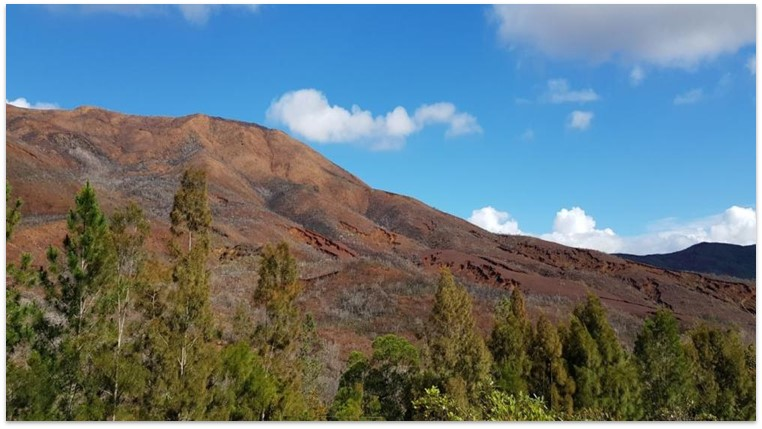
\includegraphics[width=27cm,height=16cm]{img/feux1.jpg}
        };
    \end{tikzpicture}

    %ajout de l'image supérieur
    \begin{tikzpicture}[remember picture, overlay]
        \clip [rounded corners=30pt] (-0.5cm,-2.5cm) rectangle ++(9cm,5.5cm);
        \node[inner sep=0pt, anchor=south west] at (-0.5cm,-2.5cm) { 
            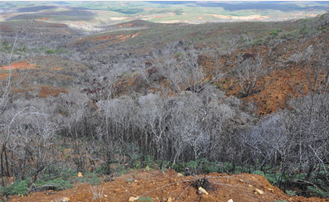
\includegraphics[width=10.5cm,height=6.5cm]{img/feux2.png}
        };
        \draw [white, line width=3pt, rounded corners=30pt] (-0.5cm,-2.5cm) rectangle ++(9cm,5.5cm); %trait blanc autour de l'image
    \end{tikzpicture}

    %ajout du versionning du rapport
    \begin{minipage}[2cm]{16cm}
        \begin{adjustwidth}{12cm}{1cm} 
            \vspace{0.5cm}
            {\fontsize{10}{12}\selectfont
            \color{version_color}
            
            }
        \end{adjustwidth}
    \end{minipage}

% intégration des titre, sous-titre, auteurs et date
    \begin{minipage}[2cm]{16cm}
        \begin{adjustwidth}{0.5cm}{1cm} 
            \vspace{2.2cm}
            {\fontsize{16}{20}\selectfont
            \color{titreColor}
            Analyse spatiale de l'impact environnemental des incendies
de 2021 sur la Nouvelle-Calédonie\\
            }

            {\fontsize{12}{14}\selectfont
            \color{grey_color}
            Hugo Roussaffa (OEIL) - J-F. N’Guyen Van Soc (OEIL) - Hélène Patel (UNC) \\
            \\
            }
    
            {\fontsize{12}{8}\selectfont
            \color{date_color}
            2024-08-12\\
            }

        \end{adjustwidth}
    \end{minipage}

    %ajout du logo OEIL
    \begin{tikzpicture}[remember picture,overlay]
        \node [inner sep=0pt] at (12.5cm,-4.8cm) {\includegraphics[width=4.5cm,height=5.5cm]{img/OEIL\_logo.png} 
        };
    \end{tikzpicture}

    %ajout d'element supplémentaire ou logo partenaire
    \begin{minipage}[1cm]{16cm}
        \begin{adjustwidth}{-0.4cm}{1cm} 
            \vspace{3.4cm}
            {\fontsize{11}{13}\selectfont
            \color{version_color}
            Diffusion Limitée - OEIL/DAVAR/DASS \\ de la Nouvelle-Calédonie\\ ou Logo partenaire/prestataire H, 5.5cm
            }
        \end{adjustwidth}
    \end{minipage}

\end{titlepage}

\renewcommand*\contentsname{Table of contents}
{
\hypersetup{linkcolor=}
\setcounter{tocdepth}{2}
\tableofcontents
}
\bookmarksetup{startatroot}

\chapter*{Preface}\label{preface}
\addcontentsline{toc}{chapter}{Preface}

\markboth{Preface}{Preface}

L'environnement est un bien commun précieux, une source de vie
inestimable, et sa préservation est une responsabilité que nous
partageons en tant que gardiens de cette planète. Dans ce contexte, la
Nouvelle-Calédonie se distingue par sa biodiversité unique et ses
écosystèmes fragiles. Cependant, elle fait face à un défi grandissant :
les incendies. Ces feux, bien qu'ils soient un phénomène naturel,
peuvent avoir des conséquences dévastatrices sur les écosystèmes
fragiles de la région. C'est dans ce contexte que l'Observatoire de
l'Environnement en Nouvelle-Calédonie (OEIL) a entrepris cette étude
approfondie pour la quatrième fois en 2021, avec pour objectif de
caractériser les incendies et de quantifier leurs impacts
environnementaux.

L'OEIL, en tant qu'institution dédiée à l'observation de l'environnement
en Nouvelle-Calédonie, s'est engagé à comprendre et à documenter les
défis environnementaux auxquels cette région unique est confrontée.
Cette étude s'inscrit dans la continuité des efforts de l'OEIL visant à
fournir des informations cruciales pour la prise de décisions éclairées
en matière de conservation de la nature et de gestion des incendies.

Ce rapport résulte d'un travail acharné, de l'expertise de nos équipes
et de la collaboration de nombreux partenaires. Il se veut une
contribution importante pour sensibiliser les décideurs, les chercheurs,
les communautés locales et le grand public à l'importance cruciale de la
préservation de l'environnement en Nouvelle-Calédonie.

À travers l'exploration des caractéristiques des incendies, de leurs
impacts sur la biodiversité, les milieux naturels, les espèces animales
et végétales, les zones protégées, la ressource en eau potable, les
surfaces agricoles, les émissions de gaz à effet de serre et les
implications financières associées à la réparation du préjudice
environnemental, ce rapport offre une vision complète des répercussions
des incendies en Nouvelle-Calédonie.

Nous espérons que cette étude contribuera à éclairer les décisions
futures en matière de préservation de l'environnement et à stimuler des
actions concrètes pour protéger ce patrimoine naturel exceptionnel.
Notre engagement envers la Nouvelle-Calédonie et son environnement
perdurera, et nous sommes convaincus que grâce à une compréhension
approfondie des défis, nous pouvons travailler ensemble pour préserver
ce joyau de la biodiversité mondiale.

Fabien Albouy Directeur de l'Observatoire de l'Environnement en
Nouvelle-Calédonie (OEIL)

\bookmarksetup{startatroot}

\chapter*{Partenaires}\label{partenaires}
\addcontentsline{toc}{chapter}{Partenaires}

\markboth{Partenaires}{Partenaires}

\begin{figure}

\begin{minipage}{\linewidth}

\includegraphics[width=1.04167in,height=\textheight]{./ressources/logos/AFD.png}

\includegraphics[width=1.04167in,height=\textheight]{./ressources/logos/ANCB.png}

\includegraphics[width=1.04167in,height=\textheight]{./ressources/logos/Endemia_CARRE.png}

\includegraphics[width=1.04167in,height=\textheight]{./ressources/logos/IAC.jpg}

\includegraphics[width=1.04167in,height=\textheight]{./ressources/logos/ifrecor.jpg}

\includegraphics[width=1.04167in,height=\textheight]{./ressources/logos/Ifremer.png}

\includegraphics[width=1.04167in,height=\textheight]{./ressources/logos/IRD_160.jpg}

\includegraphics[width=1.04167in,height=\textheight]{./ressources/logos/IUCN_Red_List.png}

\includegraphics[width=1.04167in,height=\textheight]{./ressources/logos/KBA.png}

\includegraphics[width=1.04167in,height=\textheight]{./ressources/logos/LOGO DSCGR.jpg}

\includegraphics[width=1.04167in,height=\textheight]{./ressources/logos/LOGO GOUV 300dpi.jpg}
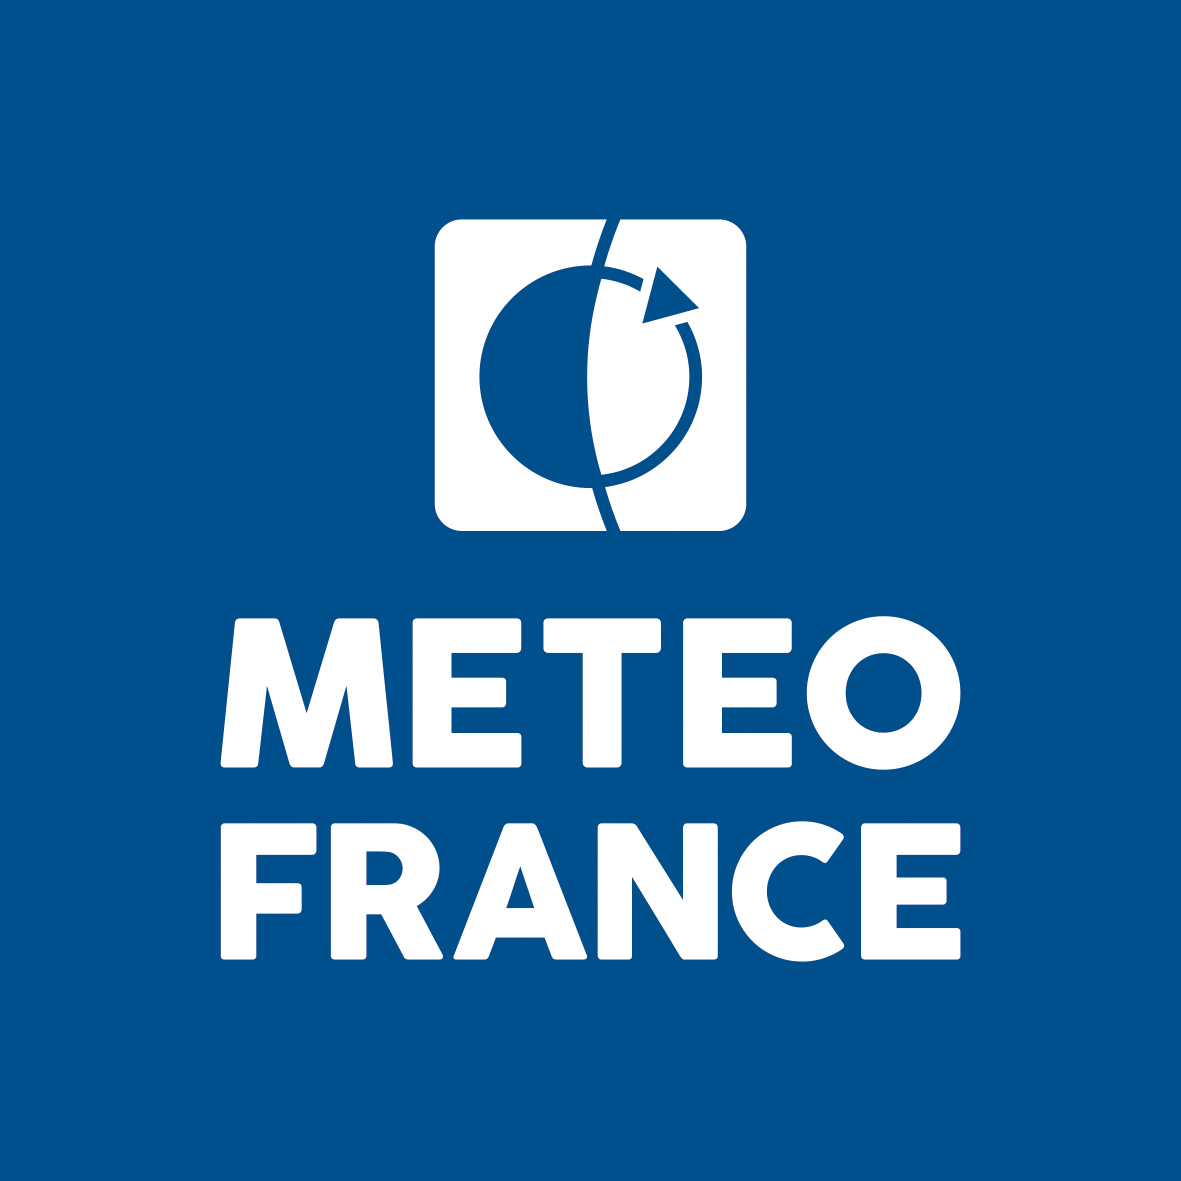
\includegraphics[width=1.04167in,height=\textheight]{./ressources/logos/METEO_France_MFBLEU-RVB.jpg}

\includegraphics[width=1.04167in,height=\textheight]{./ressources/logos/nasa_fond_blanc.jpg}
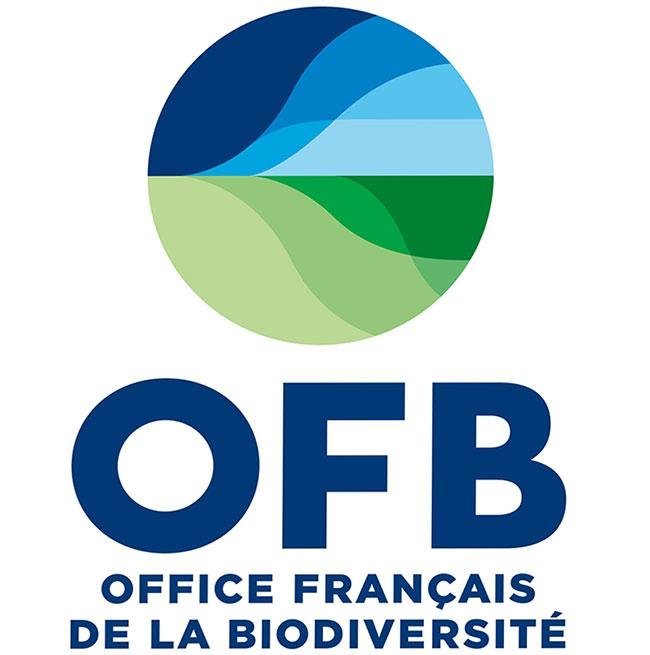
\includegraphics[width=1.04167in,height=\textheight]{./ressources/logos/OFB.jpg}
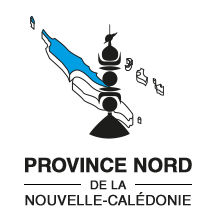
\includegraphics[width=1.04167in,height=\textheight]{./ressources/logos/Province Nord.png}

\includegraphics[width=1.04167in,height=\textheight]{./ressources/logos/province_sud.png}

\includegraphics[width=1.04167in,height=\textheight]{./ressources/logos/UNC_160.jpg}

\includegraphics[width=1.04167in,height=\textheight]{./ressources/logos/UNEP_WCMC.PNG}
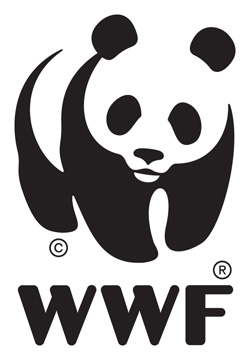
\includegraphics[width=1.04167in,height=\textheight]{./ressources/logos/wwf_panda_logo.jpg}
\includegraphics[width=1.04167in,height=\textheight]{./ressources/logos/Zonéco_NC.jpg}
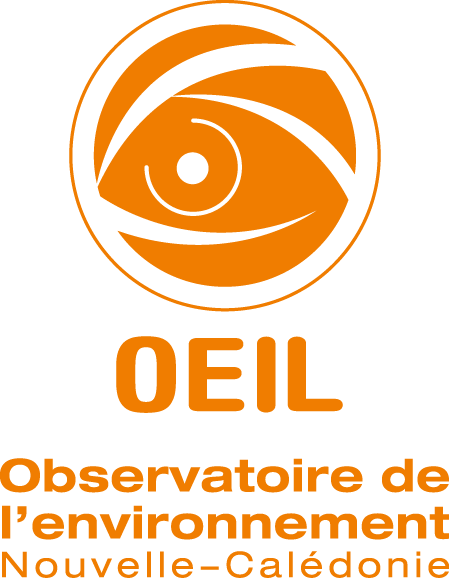
\includegraphics[width=1.04167in,height=\textheight]{./ressources/logos/OEIL.png}\end{minipage}%

\end{figure}%

\bookmarksetup{startatroot}

\chapter*{Introduction}\label{introduction}
\addcontentsline{toc}{chapter}{Introduction}

\markboth{Introduction}{Introduction}

L'Observatoire de l'Environnement en Nouvelle-Calédonie (OEIL) s'engage
dans une étude cruciale visant à caractériser les incendies survenus en
2021 en Nouvelle-Calédonie, tout en quantifiant leurs impacts
environnementaux. Cette initiative découle de la nécessité de combler un
manque criant de données concernant les incendies et leurs conséquences
sur ce territoire reconnu comme un trésor de biodiversité mondiale. La
Nouvelle-Calédonie abrite de nombreuses espèces animales et végétales
endémiques dont la survie est menacée par les changements dans leurs
habitats naturels, notamment dus aux incendies fréquents et étendus.
L'OEIL, fort de son expertise en télédétection et géomatique, s'est
engagé à caractériser cette pression environnementale et à documenter
ses impacts de manière pérenne. Les données issues des satellites
Sentinel 2 européens du programme Copernicus sont utilisées pour évaluer
les surfaces brûlées, qui sont ensuite croisées avec les informations
environnementales disponibles.

Ce rapport explore les conséquences des incendies de l'année 2021 en
Nouvelle-Calédonie, il représente la quatrième édition d'une série
d'évaluations annuelles des incendies en Nouvelle-Calédonie, débutée en
2017.

De l'impact sur la biodiversité à l'incidence sur les émissions de gaz à
effet de serre, en passant par les conséquences sur la ressource en eau
potable et les surfaces agricoles, cette étude offre une vision globale
et locale des répercussions des incendies en Nouvelle-Calédonie. La
caractérisation des surfaces brûlées constitue une étape essentielle de
l'étude, nous permettant de mieux comprendre les incendies de l'année
2021 en Nouvelle-Calédonie. Dans cette section, nous explorerons
l'analyse spatiale des surfaces brûlées en examinant leur répartition
par unité territoriale et leur distribution selon le type de foncier. De
plus, nous analysons la taille des surfaces brûlées, ainsi que leur
densité en fonction de l'historique des données disponibles. Nous
étudions également la répartition des incendies par rapport au substrat,
ce qui nous aidera à évaluer leur impact sur les écosystèmes. Enfin,
nous examinons la distance entre les zones brûlées et les sources
potentielles, ce qui nous permettra de mieux appréhender les facteurs
qui contribuent à la propagation des incendies. En parallèle, nous
abordons l'analyse temporelle, en évaluant la variabilité interannuelle
des départs de feux et en étudiant la saisonnalité des surfaces brûlées.
L'objectif final est de dresser un bilan complet de la répartition
spatio-temporelle des surfaces brûlées en Nouvelle-Calédonie.

\bookmarksetup{startatroot}

\chapter*{Résumé executif}\label{ruxe9sumuxe9-executif}
\addcontentsline{toc}{chapter}{Résumé executif}

\markboth{Résumé executif}{Résumé executif}

\section*{Objectif}\label{objectif}
\addcontentsline{toc}{section}{Objectif}

\markright{Objectif}

L'objectif de cette étude est de caractériser les incendies de l'année
2021 sur la Nouvelle-Calédonie et de quantifier les impacts
environnementaux associés en s'appuyant sur des données géographiques
relatives aux enjeux environnementaux.

\section*{Contexte}\label{contexte}
\addcontentsline{toc}{section}{Contexte}

\markright{Contexte}

L'origine de ce bilan annuel résulte du constat d'un manque de
caractérisation des incendies et, de fait, d'absence de quantification
des impacts induits par les feux sur le territoire calédonien. La
Nouvelle-Calédonie, considérée comme un haut-lieu de la biodiversité
mondiale, accueille un grand nombre d'espèces animales et végétales
endémiques voire micro-endémiques dont la survie est impactée par les
changements infligés aux milieux naturels. Les incendies, du fait de
leur ampleur et de leur fréquence, exercent une pression importante sur
ces milieux. Leurs effets peuvent être directs, mais également
indirects. L'OEIL, a développé des méthodes issues de la télédétection
et de la géomatique afin de caractériser cette pression et ses impacts
environnementaux sur l'ensemble de la Nouvelle-Calédonie. Parallèlement
aux outils numériques d'alerte et de suivi\footnote{\url{https://oeil.nc/fr/page/alerte-incendies}}
de cette pression qu'il a pu développer, L'observatoire a pour ambition
de produire un bilan détaillé annuellement afin d'inscrire la
caractérisation des incendies de manière pérenne dans le suivi des
impacts liés aux pressions environnementales.

\section*{Méthodologie}\label{muxe9thodologie}
\addcontentsline{toc}{section}{Méthodologie}

\markright{Méthodologie}

Les données sur les surfaces brûlées sont issues d'un processus de
traitement des images satellitaires issues des satellites Sentinel 2A et
2B dotés d'une résolution spatiale décamétrique. Les surfaces détectées
ont été croisées avec une vingtaine de sources d'information relatives
aux enjeux environnementaux.

\section*{Résultats et conclusions}\label{ruxe9sultats-et-conclusions}
\addcontentsline{toc}{section}{Résultats et conclusions}

\markright{Résultats et conclusions}

Ce travail représente la quatrième quantification des incendies issus
d'images hautes résolutions sur le territoire calédonien et constitue la
suite du travail engagé en 2017. Voici un extrait des résultats
obtenus~: La caractérisation du phénomène montre que 2021 est une des
années relativement moins impactées avec un total de \{\{ x \}\}
hectares incendiés, soit \{\{ x\% \}\} de la superficie de la
Nouvelle-Calédonie impactée par les feux. Ce constat est confirmé par
une analyse temporelle, où 2021 détient près de \{\{ x \% / annee n-1
\}\} en moins d'incendies par rapport à 2021, une année très impactée,
et reste comparable à 2018 avec près de 200 incendies détectés par le
capteur VIIRS. Cette année est considérée selon Météo France comme une
année pluvieuse suite à l'influence du phénomène la Nina. En
s'intéressant à la saisonnalité des feux, selon les données du capteur
VIIRS, il n'y a que le mois de janvier 2020 qui reste supérieur à la
médiane mensuelle sur la période 2012-2020. Ce constat est également
souligné par Météo France dans son bulletin climatique annuel où il y a
eu un déficit pluviométrique sur le mois de janvier 2020. Sur le reste
de l'année, le cumul des incendies reste faible par rapport aux médianes
mensuelles 2012-2020, en correspondance avec l'analyse réalisée par
Météo France, avec six épisodes pluviométriques marquants dans l'année,
deux phénomènes cycloniques, avec un mois de décembre ayant un bilan
pluviométrique largement excédentaire. Près de 88\% des surfaces brûlées
en 2020 concernent des secteurs jamais incendiés en comparaison avec les
années précédentes entre 2017 et 2019. La répartition spatiale de ces
incendies reste hétérogène sur le territoire calédonien avec une grande
partie Nord de la Grande Terre plus touchée, et notamment la Province
Nord qui reste la province la plus touchée avec près de 58\% de la
superficie impactée. La commune de Boulouparis reste la plus impactée
avec près de 1 566 hectares brûlés. L'aire coutumière Hot ma whaap,
constituée de trois communes les plus impactées par les incendies
dépassant les 1000 hectares (Ouégoa, Kaala Gomen et Voh) concerne à elle
seule près de 40\% de la superficie brûlée en Nouvelle-Calédonie. Cette
répartition correspond également aux résultats sur le substrat, où il
s'agit du sol utramafique qui a été le plus impacté réparti
essentiellement sur les 5 communes les plus impactées (Boulouparis,
Kaala-Gomen, Ouégoa, Voh, Pouembout) avec plus de 5 000 hectares, soit
près de 30\% de la superficie incendiée en Nouvelle-Calédonie. Il est
constaté que 80\% des incendies se produisent à moins de 500 mètres
d'une voie d'accès et ce sont près de 70\% des incendies se produisent à
moins d'un kilomètre d'une habitation ou d'une construction. En
considérant la taille des zones brûlées sur l'année 2020, celles-ci sont
en grande partie de petite taille, plus de 90\% ne dépassant pas les 10
hectares. Avec une année assez humide, ces petites surfaces brûlées ont
été plus nombreuses et participent à plus de 50\% de la superficie
totale brûlée.

Ainsi les impacts qui en découlent sont conséquents. La destruction du
couvert végétal est estimée à 11 936 hectares soit 3 fois moins qu'en
2019. De façon plus détaillée, la répartition pour 100 hectares de
végétation brûlés, 47 hectares ont concerné la strate de végétation
arbustive, 39 hectares pour la strate herbacée, et 14 hectares pour la
strate arborée. La strate de végétation arbustive a donc été
principalement impactée avec plus de 5 000 hectares, chiffre inférieur à
2019 mais supérieure à 2018, année moins impactée. La végétation
arborée, dont font partie les forêts qui représentent les écosystèmes
les plus riches, a subi tout de même des dégâts avec plus de 1000
hectares mais c'est deux fois moins qu'en 2019. Parmi la végétation, des
écosystèmes particuliers (forêts sèches, mangroves) ont également été
impactées 2020. Les zones de vigilance concernant les forêts sèches ont
brûlée sur 26 hectares, moins de 15 hectares qu'en 2019. Les mangroves,
ont été impactés à près de 60 hectares.

Au sein de ces formations végétales, des espèces endémiques, souvent
rares et menacées, sont potentiellement impactées. En considérant les
périmètres d'alerte sur les espèces menacées, 326 d'entre eux ont été
très certainement touchés par les flammes, dont 60\% concernent des
espèces classées en danger d'extinction selon les critères de l'UICN.
Dans les faits, ces périmètres d'alerte concernent 124 espèces.

Certaines aires géographiques présentant un intérêt écologique et
biologique bénéficient d'une protection réglementaire ou d'un label
international. Ces périmètres protégés ont subi des impacts plus
conséquents en 2019 que les deux années précédentes. Concernant les
zones tampons de l'UNESCO, plus de 4 600 hectares ont été incendiés en
2020. Parmi les aires protégées provinciales terrestres, 14 d'entre
elles ont été impactées sur une superficie de plus de 250 hectares.

Les incendies de 2020 ont également impacté la ressource en eau, avec
120 périmètres de protection des eaux touchés (soit 19\% des périmètres
de protection des eaux du territoire) sur près de 2 500 hectares. Les
incendies sur terres agricoles ont concerné plus de 1 400 hectares
brûlés, dont 80\% concerne sans surprise des zones de pâturage, le
secteur de l'élevage étant le plus représenté en Nouvelle-Calédonie. En
utilisant l'outil OCMC, il a été possible d'estimer à 55 milliards de F
CFP le coût de la restauration écologique relatif aux impacts sur la
végétation et les écosystèmes associés. En utilisant ainsi la méthode
déterminée par le GIEC, les émissions de gaz à effet de serre sont
évaluées à 232 637 teq CO2, représentant environ 3\% des émissions à
l'échelle de la Nouvelle-Calédonie.

\section*{Limites de l'étude}\label{limites-de-luxe9tude}
\addcontentsline{toc}{section}{Limites de l'étude}

\markright{Limites de l'étude}

Bien qu'aucun autre bilan n'ait été réalisé en Nouvelle-Calédonie avec
un tel niveau de précision, il présente quelques limites liées aux
données sur les incendies. En effet, la détection exclusive des surfaces
brûlées par les satellites possède des biais liés à la présence de
nuages et à d'autres objets pouvant être confondus avec des surfaces
brûlées (végétation sèche, labours, \ldots). De même, la procédure de
contrôle des incendies détectés par Sentinel 2 a nécessité des prises de
décisions qui possèdent leurs limites (contrôle automatique par un mode
d'occupation du sol datant de 2014 et à une résolution différente de
celles des données sur les incendies, des erreurs potentielles lors de
la classification des surfaces détectées durant la phase de
photo-interprétation, \ldots). Par ailleurs, les données utilisées pour
caractériser l'impact des incendies possèdent elles aussi des facteurs
intrinsèques qui peuvent limiter leur utilisation (échelle de travail
différente de celles des données sur les incendies, données non
exhaustives, \ldots).

\bookmarksetup{startatroot}

\chapter*{Glossaire}\label{glossaire}
\addcontentsline{toc}{chapter}{Glossaire}

\markboth{Glossaire}{Glossaire}

\begin{longtable}[]{@{}
  >{\raggedright\arraybackslash}p{(\columnwidth - 2\tabcolsep) * \real{0.1838}}
  >{\raggedright\arraybackslash}p{(\columnwidth - 2\tabcolsep) * \real{0.8162}}@{}}
\toprule\noalign{}
\begin{minipage}[b]{\linewidth}\raggedright
Terme
\end{minipage} & \begin{minipage}[b]{\linewidth}\raggedright
Définition
\end{minipage} \\
\midrule\noalign{}
\endhead
\bottomrule\noalign{}
\endlastfoot
Biomasse & Matière organique d'origine végétale (microalgues incluses),
animale, bactérienne ou fongique, utilisable comme source d'énergie
(bioénergies). \\
Chaine de traitement & Succession des opérations effectuées sur les
données à l'aide de scripts et outils développés avec un ou plusieurs
produits en sortie. \\
Couche & Fichier contenant les données spatiales en ayant les
informations attributaires / tabulaires. \\
Discrétisation & Méthode permettant de découper en classe une série de
variables quantitatives ou qualitatives. \\
Héliophile & Organisme ayant d'importants besoins en lumière (soleil)
pour se développer. \\
Photo-interprétation & Interprétation et vérification à partir de
photographies aériennes ou d'images satellitales. \\
Pyrophile & Plante ou végétation se développant sur un substrat ayant
subi un incendie. \\
Raster & L'information est traitée sous forme de valeur numérique et
correspond souvent à une image géoréférencée. \\
Signature spectrale & Émission électromagnétique caractéristique d'un
objet en fonction de la longueur d'onde. \\
\end{longtable}

\bookmarksetup{startatroot}

\chapter*{Sources de données exploitées dans
l'étude}\label{sources-de-donnuxe9es-exploituxe9es-dans-luxe9tude}
\addcontentsline{toc}{chapter}{Sources de données exploitées dans
l'étude}

\markboth{Sources de données exploitées dans l'étude}{Sources de données
exploitées dans l'étude}

En accord avec les acteurs de l'environnement en Nouvelle-Calédonie, des
données environnementales ont été mise à disposition de l'OEIL afin de
caractériser l'impact des incendies sur les milieux. Ainsi, des
traitements ont été effectués en utilisant ces données afin de pouvoir
quantifier le nombre d'incendies et la superficie incendiée pour chaque
source d'information étudiée. Le Table~\ref{tbl-source-impact} présente
les informations étudiées ainsi que leurs principales caractéristiques.

\newpage{}

\KOMAoptions{paper=landscape,pagesize}
\recalctypearea

\newpage
\newgeometry{top=20mm,left=20mm,right=-60mm,bottom=120mm}

\begin{table}

\caption{\label{tbl-source-impact}Présentation des sources d'information
utilisées pour réaliser le bilan de l'impact des incendies}

\centering{

\href{C:/Users/oriane.bruyere/projets/output_bilan/data_sources/tbl-source-impact-environnement.html}{\includegraphics{C:/Users/oriane.bruyere/projets/output_bilan/data_sources/tbl-source-impact-environnement.png}}

}

\end{table}%

\KOMAoptions{paper=landscape,pagesize}
\recalctypearea

\newpage
\newgeometry{top=20mm,left=20mm,right=-60mm,bottom=120mm}

\href{C:/Users/oriane.bruyere/projets/output_bilan/data_sources/tbl-source-impact-agrigulture.html}{\includegraphics{C:/Users/oriane.bruyere/projets/output_bilan/data_sources/tbl-source-impact-agrigulture.png}}

\href{C:/Users/oriane.bruyere/projets/output_bilan/data_sources/tbl-source-impact-interet.html}{\includegraphics{C:/Users/oriane.bruyere/projets/output_bilan/data_sources/tbl-source-impact-interet.png}}

\href{C:/Users/oriane.bruyere/projets/output_bilan/data_sources/tbl-source-impact-ress-eau.html}{\includegraphics{C:/Users/oriane.bruyere/projets/output_bilan/data_sources/tbl-source-impact-ress-eau.png}}

\KOMAoptions{paper=landscape,pagesize}
\recalctypearea

\newpage
\newgeometry{top=20mm,left=20mm,right=-60mm,bottom=120mm}

\href{C:/Users/oriane.bruyere/projets/output_bilan/data_sources/tbl-source-impact-feux.html}{\includegraphics{C:/Users/oriane.bruyere/projets/output_bilan/data_sources/tbl-source-impact-feux.png}}

\href{C:/Users/oriane.bruyere/projets/output_bilan/data_sources/tbl-source-impact-feux2.html}{\includegraphics{C:/Users/oriane.bruyere/projets/output_bilan/data_sources/tbl-source-impact-feux2.png}}

\href{C:/Users/oriane.bruyere/projets/output_bilan/data_sources/tbl-source-impact-substrat.html}{\includegraphics{C:/Users/oriane.bruyere/projets/output_bilan/data_sources/tbl-source-impact-substrat.png}}

\href{C:/Users/oriane.bruyere/projets/output_bilan/data_sources/tbl-source-impact-foncier.html}{\includegraphics{C:/Users/oriane.bruyere/projets/output_bilan/data_sources/tbl-source-impact-foncier.png}}

\newpage{}

\KOMAoptions{paper=portrait,pagesize}
\recalctypearea

\newpage
\newgeometry{top=20mm,left=20mm,right=20mm,bottom=40mm}

\bookmarksetup{startatroot}

\chapter{Présentation de l'étude}\label{pruxe9sentation-de-luxe9tude}

\section{Contexte}\label{sec-contexte}

L'étude de l'impact environnemental des incendies en Nouvelle-Calédonie
résulte du constat d'un manque de caractérisation du phénomène en
lui-même et, de fait, d'absence de quantification des impacts induits
par les feux sur le territoire calédonien. La Nouvelle-Calédonie,
considérée comme un haut-lieu de la biodiversité mondiale, est composée
d'espèces animales et végétales dont la survie est impactée par les
changements infligés aux milieux naturels. Les incendies, du fait de
leur ampleur et de leur fréquence, exercent une pression considérable
sur ces milieux. Leurs effets peuvent être directs, mais également
indirects. Le feu est susceptible d'affecter les populations des espèces
endémiques et, micro-endémiques. Le passage des incendies en brûlant la
végétation, rend les sols plus sensibles à l'érosion. L'érosion provoque
un apport supplémentaire en matériaux aux cours d'eaux puis au lagon,
avec une altération de la qualité des milieux. L'ouverture des milieux
induite par les incendies est souvent favorable au développement des
espèces envahissantes végétales et animales. Les incendies contribuent à
la fragmentation des milieux notamment en accentuant l'effet de lisière.
De plus, les émanations gazeuses liées à la combustion ont une influence
directe sur la qualité de l'air et contribuent aux changements globaux.
In fine, ce sont l'ensemble des services rendus par les écosystèmes qui
peuvent être altérés par les incendies. Ainsi, l'identification, la
quantification et le suivi des surfaces incendiées sont nécessaires pour
rendre compte de l'impact de ces derniers sur l'environnement. La base
de données sur les surfaces incendiées pourrait également servir à
consolider les stratégies de luttes contre les incendies, aiguiller la
gestion du patrimoine naturel et enfin être prise en compte dans
l'aménagement du territoire.

C'est dans une démarche de caractérisation de la pression
environnementale liée aux incendies et de ses impacts, que l'OEIL a
entrepris des études dès 2013 \footnote{\url{https://www.oeil.nc/cdrn/index.php/resource/bibliographie/view/5769}}
sur la faisabilité de mise en place d'un suivi des incendies via les
outils de télédétection et sur les indicateurs qui pourraient être
renseignés. Des premiers travaux ont conduit à mettre en production et à
optimiser une chaîne de traitement dans le cadre du projet INC
(Incendies et biodiversité de écosystèmes en Nouvelle-Calédonie)
\footnote{Projet de recherche financé par l'Agence Nationale de la
  Recherche, coordonné par Christelle Hély-Alleaume du CRNS. Les
  partenaires du projet sont : l'IRSTEA (ancien CEMAGREF), l'INRA,
  l'IRD, Météo France et le CRNS.}. Ce traitement automatisé permet
d'exploiter les données d'anomalies thermiques provoquées par les feux
et détectées par les satellites. Ce processus s'appuie sur un service
déjà existant de la National Aeronautics and Space Administration (NASA)
qui intègre les informations de trois satellites : Aqua MODIS, Terra
MODIS et Suomi NPP, ainsi que sur les données du satellite Himawari de
la Japan Meteorological Agency (JAXA). Depuis début 2018, l'efficacité
de ce processus a permis de mettre à la disposition de tous, un système
d'alerte sur les incendies \footnote{Pour s'abonner à ce système
  d'alerte, cliquer sur ce lien
  \url{https://oeil.nc/AlerteIncendies/AbonnezVous}}. Ce service permet
de recevoir une alerte par courriel à chaque nouvelle détection, est
couplé au géoportail VULCAIN \footnote{Cliquez sur
  \url{https://geoportail.oeil.nc/AlerteIncendies/} pour accéder au
  portail.} qui, outre la localisation de l'incendie en cours, permet
d'analyser la chronique des données « Incendies » et de produire ses
propres analyses thématiques. Dans le cadre de cette étude, pour
réaliser une analyse temporelle, il est nécessaire de s'appuyer sur ces
données ayant une chronique de données relativement conséquente.

La haute fréquence de revisite des satellites impliqués font de ces
données une source fiable pour fournir des alertes sur les incendies en
cours. En revanche, le manque de précision des données de surfaces
potentiellement brûlées générées à partir de ces anomalies thermiques
(pixel le plus fin de 375 mètres \footnote{\url{https://geoportail.oeil.nc/geoportal/catalog/search/resource/details.page?uuid=\%7B5D28AFE1-541C-4102-84F0-6959F769FA78\%7D}}),
a encouragé l'OEIL à travailler sur des données satellitaires plus
précises issues des satellites Sentinel 2 qui offrent une résolution de
spatiale de 10 mètres. En effet, la méthode d'analyse des images
satellitaires issues des satellites Sentinel 2 et la précision accrue
des données permet d'être plus exhaustif et beaucoup plus précis quant
aux contours de surfaces brulées. Cette méthode est détaillée en dans le
rapport méthodologique \textbf{?@sec-methodosentinel2}. Les résultats
générés étant les plus pertinents pour une quantification des surfaces
brûlées et des impacts environnementaux, ils seront utilisés dans le
présent rapport.

Les acteurs de l'environnement en Nouvelle-Calédonie produisent, selon
leurs champs d'intervention, un certain nombre d'informations permettant
de caractériser l'environnement. En accord avec ces derniers, des
données ont été fournies à l'OEIL afin de déterminer l'impact de la
superficie brûlée sur les milieux néo-calédoniens depuis 2017.

\section{Périmètre spatial et temporel de
l'étude}\label{puxe9rimuxe8tre-spatial-et-temporel-de-luxe9tude}

Souhaitant établir une caractérisation, et quantification globale des
impacts induits par les feux, l'Observatoire a privilégié la détection
des zones brûlées sur une année complète et sur l'ensemble du
territoire.

Avant cela, et ce malgré l'ampleur de la problématique, seuls la
Direction de la Sécurité Civile et de la Gestion des Risques (DSCGR) et
les sapeurs-pompiers réalisaient un suivi des incendies, mais de manière
ponctuelle et de précisions hétérogènes imprécise , ce qui ne suffisait
pas à établir un bilan complet de l'impact des incendies. En effet, ce
suivi est peu précis en termes de localisation des évènements et ne
retrace par l'empreinte exacte de l'incendie. La DSCGR réalise également
des missions aériennes d'identification des incendies, lorsqu'un plan
ORSEC est déclenché, notamment lorsque plusieurs communes sont touchées
simultanément.

\section{Objectif}\label{objectif-1}

L'objectif principal du présent rapport est de pouvoir caractériser à
partir de données satellitaire la pression des incendies et de
quantifier leur impact environnemental sur l'année 2021, à partir des
données d'enjeux environnementaux produites par les partenaires de
l'OEIL en Nouvelle-Calédonie.

\bookmarksetup{startatroot}

\chapter{Méthode de production des
résultats}\label{muxe9thode-de-production-des-ruxe9sultats}

Les données sur les incendies utilisées dans le cadre de cette étude,
décrite dans la partie~\ref{sec-contexte}, ainsi que leurs méthodes de
production sont détaillées en \textbf{?@sec-appendix-datasources}.

Afin de mesurer les impacts environnementaux qui découlent des
incendies, de nombreuses données exogènes ont pu être considérées dans
cette étude Table~\ref{tbl-source-impact} .

\bookmarksetup{startatroot}

\chapter{Caractérisation des zones
brulées}\label{caractuxe9risation-des-zones-bruluxe9es}

Dans cette partie du rapport sont présentées des données chiffrées
permettant de caractériser les incendies sur le territoire calédonien à
différentes échelles temporelles et spatiales.

Le nombre de surfaces brûlées ainsi que les superficies incendiées en
2021 en Nouvelle-Calédonie sont regroupés par perimètres administratifs
puis par type de foncier. Une analyse spatiale des incendies met en
avant les secteurs qui regroupent le plus grand nombre de zones brûlées
et les secteurs ayant les plus grandes surfaces incendiés. Pour
compléter, une analyse de la taille des surfaces brûlées est réalisée
afin de déterminer celles qui contribuent le plus à la superficie
incendiée sur le territoire. Enfin, pour avoir quelques facteurs
descriptifs des zones brûlées, une analyse est réalisée en fonction du
type de substrat ainsi qu'une étude de la proximité des incendies aux
habitations et aux voies d'accès permettant d'étudier le lien entre
incendies et la présence d'infrastructures humaines.

\section{Analyse spatiale des surfaces
brûlées}\label{analyse-spatiale-des-surfaces-bruxfbluxe9es}

Cette partie du rapport présente différentes approches ayant pour but de
caractériser la répartition des zones brûlées tout en tenant compte
d'autres facteurs comme le substrat ou zones anthropiques à proximité
des surfaces brûlées. Leur taille et leur localisation sont prises en
compte afin de mettre en avant les lieux où les incendies ont été les
plus intenses.

\subsection{Répartition par unité
territoriale}\label{ruxe9partition-par-unituxe9-territoriale}

Sont présentés dans cette partie, le nombre d'incendies et la superficie
en hectares incendiés par unité administrative. Ces résultats s'appuient
principalement sur les données issues de la chaîne de traitement des
images satellitaires de Sentinel 2.

\subsubsection{Répartition en
Nouvelle-Calédonie}\label{ruxe9partition-en-nouvelle-caluxe9donie}

À l'échelle de la Nouvelle-Calédonie, les résultats sont présentés pour
les données du capteur VIIRS du satellite SUOMI NPP et sur les données
issues de la chaîne de traitement des images satellitaires de Sentinel
2.

\paragraph{Informations}\label{informations}

\begin{figure}[H]

\centering{

\href{C:/Users/oriane.bruyere/projets/output_bilan/etude_caracterisation/fig-zb-nc.html}{\includegraphics{C:/Users/oriane.bruyere/projets/output_bilan/etude_caracterisation/fig-zb-nc.png}}

}

\caption{\label{fig-zb-nc}Carte de l'impact des surfaces brûlées sur la
Nouvelle-Calédonie en 2020}

\end{figure}%

Les méthodes de détections des surfaces brûlées ne sont pas les mêmes
pour ces deux satellites. Le capteur VIIRS du satellite SUOMI NPP
s'appuie sur une détection de points chauds à la surface de la terre
possédant une résolution spatiale de 375 mètres, et ce, en pointant le
pixel concerné par une augmentation de la chaleur. Le point chaud est
représenté par un pixel de 375 mètres de côté, ainsi on a une
exagération de la superficie des surfaces incendiées issues du capteur
VIIRS en comparaison avec leur taille réelle. La chaîne de traitement
des images satellitaires s'appuie quant à elle sur des images Sentinel 2
possédant au mieux 10 mètres de résolution spatiale. A la différence du
capteur VIIRS, les détections ne correspondent pas à des anomalies
thermiques, mais elles se basent en partie sur l'analyse de l'activité
chlorophyllienne de la végétation. Les surfaces détectées par Sentinel 2
sont donc plus précises en termes de localisation, et de superficie. Il
est tenu de souligner que la chaîne de traitement des images
satellitaires de Sentinel 2 possède des limites qui induisent une
sous-estimation probable de la superficie des surfaces incendiées
\textbf{?@sec-methodosentinel2}. Ces différences de méthodologie
expliquent que les quantifications en nombre des surfaces brûlées et en
hectares de surfaces brûlées ne soient pas exactement les mêmes
\footnote{Pour plus de détails, se référer à la partie 1 du guide
  méthodologique en appendices}.

Une localisation des zones brûlées issus de Sentinel 2 peut être
observée sur la Figure~\ref{fig-zb-nc}.

\paragraph{Résultats}\label{ruxe9sultats}

\begin{table}

\caption{\label{tbl-stats-feux-nc}Résultats des zones brûlées (Sentinel
2) en Nouvelle-Calédonie pour l'année 2020}

\centering{

\href{C:/Users/oriane.bruyere/projets/output_bilan/etude_caracterisation/tbl-stats-feux-nc.html}{\includegraphics{C:/Users/oriane.bruyere/projets/output_bilan/etude_caracterisation/tbl-stats-feux-nc.png}}

}

\end{table}%

\begin{table}

\caption{\label{tbl-stats-viirs-nc}Statistiques des zones
potentiellement incendiées détectées par le capteur VIIRS SNPP en
Nouvelle-Calédonie pour l'année 2020}

\centering{

\href{C:/Users/oriane.bruyere/projets/output_bilan/etude_caracterisation/tbl-stats-viirs-nc.html}{\includegraphics{C:/Users/oriane.bruyere/projets/output_bilan/etude_caracterisation/tbl-stats-viirs-nc.png}}

}

\end{table}%

\begin{figure}[H]

\centering{

\href{C:/Users/oriane.bruyere/projets/output_bilan/etude_caracterisation/fig-diag-zb-new.html}{\includegraphics{C:/Users/oriane.bruyere/projets/output_bilan/etude_caracterisation/fig-diag-zb-new.png}}

}

\caption{\label{fig-diag-zb-new}Comparaison de la superficie déjà
incendiée en fonction des résultats précédents de 2017 à 2020}

\end{figure}%

\subsubsection{Répartition par
province}\label{ruxe9partition-par-province}

\begin{figure}[H]

\centering{

\href{C:/Users/oriane.bruyere/projets/output_bilan/etude_caracterisation/fig-part-sb-province.html}{\includegraphics{C:/Users/oriane.bruyere/projets/output_bilan/etude_caracterisation/fig-part-sb-province.png}}

}

\caption{\label{fig-part-sb-province}Part de la superficie brûlée par
province en 2020}

\end{figure}%

\begin{table}

\caption{\label{tbl-stats-feux-province}Répartition par province des
zones brûlées pour l'année 2020}

\centering{

\href{C:/Users/oriane.bruyere/projets/output_bilan/etude_caracterisation/tbl-stats-feux-province.html}{\includegraphics{C:/Users/oriane.bruyere/projets/output_bilan/etude_caracterisation/tbl-stats-feux-province.png}}

}

\end{table}%

\begin{figure}[H]

\centering{

\href{C:/Users/oriane.bruyere/projets/output_bilan/etude_caracterisation/fig-graph-evol-feux-province.html}{\includegraphics{C:/Users/oriane.bruyere/projets/output_bilan/etude_caracterisation/fig-graph-evol-feux-province.png}}

}

\caption{\label{fig-graph-evol-feux-province}Evolution de la superficie
brûlée (Sentinel 2) de 2017 à 2020 par province}

\end{figure}%

\subsubsection{Répartition par
commune}\label{ruxe9partition-par-commune}

\begin{figure}[H]

\centering{

\href{C:/Users/oriane.bruyere/projets/output_bilan/etude_caracterisation/fig-carte-choro-feux-commune.html}{\includegraphics{C:/Users/oriane.bruyere/projets/output_bilan/etude_caracterisation/fig-carte-choro-feux-commune.png}}

}

\caption{\label{fig-carte-choro-feux-commune}Part de la superficie
brûlée par commune en 2020}

\end{figure}%

\begin{table}

\caption{\label{tbl-stat-feux-commune}Répartition par commune des zones
brûlées pour l'année 2020}

\centering{

\href{C:/Users/oriane.bruyere/projets/output_bilan/etude_caracterisation/tbl-stat-feux-commune.html}{\includegraphics{C:/Users/oriane.bruyere/projets/output_bilan/etude_caracterisation/tbl-stat-feux-commune.png}}

}

\end{table}%

\begin{figure}[H]

\centering{

\href{C:/Users/oriane.bruyere/projets/output_bilan/etude_caracterisation/fig-histo-cumul-feux-commune.html}{\includegraphics{C:/Users/oriane.bruyere/projets/output_bilan/etude_caracterisation/fig-histo-cumul-feux-commune.png}}

}

\caption{\label{fig-histo-cumul-feux-commune}Cumul de la superficie
brûlée entre 2017 et 2020 par commune}

\end{figure}%

\subsubsection{Répartition par aire
coutumière}\label{ruxe9partition-par-aire-coutumiuxe8re}

\begin{figure}[H]

\centering{

\href{C:/Users/oriane.bruyere/projets/output_bilan/etude_caracterisation/fig-carte-choro-feux-aire_coutumiere.html}{\includegraphics{C:/Users/oriane.bruyere/projets/output_bilan/etude_caracterisation/fig-carte-choro-feux-aire_coutumiere.png}}

}

\caption{\label{fig-carte-choro-feux-aire\_coutumiere}Part de la
superficie brûlée par aire coutumière en 2020}

\end{figure}%

\begin{table}

\caption{\label{tbl-stat-feux-aire\_coutumiere}Répartition par aire
coutumière des surfaces brûlées pour l'année 2020}

\centering{

\href{C:/Users/oriane.bruyere/projets/output_bilan/etude_caracterisation/tbl-stat-feux-aire_coutumiere.html}{\includegraphics{C:/Users/oriane.bruyere/projets/output_bilan/etude_caracterisation/tbl-stat-feux-aire_coutumiere.png}}

}

\end{table}%

\begin{figure}[H]

\centering{

\href{C:/Users/oriane.bruyere/projets/output_bilan/etude_caracterisation/fig-graph-evol-feux-aire_coutumiere.html}{\includegraphics{C:/Users/oriane.bruyere/projets/output_bilan/etude_caracterisation/fig-graph-evol-feux-aire_coutumiere.png}}

}

\caption{\label{fig-graph-evol-feux-aire\_coutumiere}Evolution de la
superficie brûlée entre 2017 et 2020 par aire coutumière}

\end{figure}%

\subsubsection{Répartition par carroyage
DFCI}\label{ruxe9partition-par-carroyage-dfci}

Le carroyage DFCI (Défense de la Forêt Contre les Incendies) est souvent
utilisé par les services de lutte contre les feux (DSCGR,
Sapeurs-pompiers) pour repérer rapidement l'emplacement d'un évènement
de type feu de forêt. Une analyse est donc fournie pour déterminer quels
carrés ont donc été les plus impactés durant l'année.

Les résultats chiffrés sont présentés en annexe dans la partie
«Répartition par unité territoriale -- Carroyage DFCI\,».

\begin{figure}[H]

\centering{

\href{C:/Users/oriane.bruyere/projets/output_bilan/etude_caracterisation/fig-carte-cloro-feux-dfci.html}{\includegraphics{C:/Users/oriane.bruyere/projets/output_bilan/etude_caracterisation/fig-carte-cloro-feux-dfci.png}}

}

\caption{\label{fig-carte-cloro-feux-dfci}Part de la superficie brûlée
en 2020 par carré du carroyage DFCI à 20 kilomètres}

\end{figure}%



\end{document}
